% Compile from the repository root with python docs/build_preliminary_report.py.
% IEEEtran provides the IEEE two-column body; the requested cover is separate.
\documentclass[conference,10pt]{IEEEtran}
\usepackage{amsmath}
\usepackage{graphicx}
\usepackage{url}
\graphicspath{{docs/assets/}}

\begin{document}
\begin{titlepage}
\thispagestyle{empty}
\begin{center}
\vspace*{1.0in}
{\large IIITS\par}
\vspace{0.65in}
{\Huge\bfseries Computer Vision Autonomous Patrol Simulator\par}
\vspace{0.26in}
{\LARGE Preliminary Project Report\par}
\vspace{0.42in}
{\large Computer Vision and Explainable Navigation\par}
\vfill
\begin{tabular}{rl}
Author: & Charanpreet Singh\\[0.12in]
Status: & Student\\[0.12in]
Student ID: & OMIO25S00012\\[0.12in]
Affiliation: & IIITS\\[0.12in]
Submission date: & 4 October 2026\\
\end{tabular}
\vspace{0.65in}
\end{center}
\noindent\textbf{Document status:} Preliminary. The implementation and tests described below are complete as of 3 October 2026; real-footage evaluation and final packaging are scheduled before submission.
\end{titlepage}

\begin{abstract}
Camera-based object detection identifies obstacles but does not directly explain how a navigation system should respond. This project develops a software-only patrol simulator that converts webcam or video frames into an inspectable straight, turn, or stop recommendation. The current prototype combines an optional Ultralytics YOLO11n detector, a class-aware intersection-over-union tracker, horizontal navigation zones, an image-space collision corridor, approximate monocular distance bands, per-object risk scores, and left/right corridor aggregation. A PySide6 dashboard presents annotated frames, the selected action and reason, steering angle, simulated wheel speeds, risk map, and telemetry. The implementation is modular and configurable through YAML. Initial verification on 3 October 2026 found that all six headless navigation tests pass; the installed model loads on CPU; and the 24-second synthetic demonstration video yields no YOLO detections at five sampled times. Controlled injected-detection scenes nevertheless exercise the downstream turn and stop logic and are labeled as such. These results establish a working decision prototype, not detection accuracy or safe autonomous operation. Before the 4 October 2026 submission, the remaining work is to run a small real-footage check, document observed inference behavior and limitations, verify the final demonstration, and package the code and report. Future improvements include camera calibration, stronger tracking, and consistency fixes for corridor display and stop handling.
\end{abstract}
\begin{IEEEkeywords}
computer vision, object detection, monocular distance, risk assessment, explainable navigation, simulation
\end{IEEEkeywords}

\section{Introduction}
\subsection{Background and Purpose}
Detecting a person or vehicle is only the first step in visual navigation. A camera-based application must also decide whether the object lies near a projected route, whether another route appears less occupied, and when to stop. General object-detection datasets such as COCO address recognition and localization in complex scenes \cite{coco}; they do not, by themselves, define a safe navigation policy. This project therefore focuses on the transparent transformation from image observations to a \emph{simulated} decision. It does not drive hardware.

The operational goal is to accept webcam or recorded video, detect configured object classes when a model is available, attach stable identities to detections, estimate image-space position and rough proximity, combine scene risks, and display the resulting recommendation together with its reason. The user should be able to replay a scenario, inspect the intermediate overlays, and compare the left and right corridor scores.

\subsection{Objectives and Boundaries}
The specific objectives are to (1) build a repeatable capture and detection path, (2) associate detections across frames, (3) evaluate approximate proximity and navigation zones, (4) choose a lower-risk route or stop based on multiple objects, and (5) expose each stage in a desktop dashboard and log. The boundary is important: a single uncalibrated RGB camera does not supply reliable metric depth, and the wheel values are display outputs, not commands to an actuator. No mapping, localization, or roadworthiness claim is made.

\section{Progress to Date and Methodology}
\subsection{Implemented Pipeline}
The application currently uses OpenCV capture for a webcam or MP4 file. A configurable Ultralytics YOLO11n model \cite{yolo11} accepts each frame with default confidence and non-maximum-suppression IoU parameters of 0.45 and an inference size of 640 pixels. The adapter retains the configured classes: person, bicycle, car, motorcycle, bus, truck, and chair. If the model is disabled or cannot load, the interface remains usable but returns no detections. The detector is based on a COCO-pretrained model according to the vendor documentation \cite{yolo11}; no project-specific model training has been performed.

The custom tracker matches same-class detections to existing tracks by bounding-box IoU, with a default matching threshold of 0.25 and a 12-frame missing-track allowance. Its area history labels apparent approach or retreat. This tracker is intentionally simpler than published tracking-by-detection systems such as SORT, which additionally use prediction and assignment machinery \cite{sort}; SORT performance numbers are not attributed to this implementation.

Each detection is assigned to one of five equally spaced horizontal zones by its box center. A separate central image-space corridor test increases the risk of objects whose centers fall in the projected path. Distance is approximated by
\begin{equation}
  \widehat{d}=\frac{f_{\mathrm{px}}H_{\mathrm{prior}}}{h_{\mathrm{box}}},
\end{equation}
where $f_{\mathrm{px}}$ defaults to 700 pixels, $H_{\mathrm{prior}}$ is an assumed height for the detected class, and $h_{\mathrm{box}}$ is bounding-box height. The result is categorized as safe, caution, near, or critical using the configured thresholds of 6, 4, and 2~m. This pinhole-style relationship depends on camera calibration and object geometry \cite{opencvcalib}; the displayed value is explicitly labeled an estimate.

The heuristic per-object risk combines proximity, normalized box area, lower-frame position, corridor membership, class weight, confidence, and an approach bonus. The highest risk in each zone forms a zone score. Left and right zone scores are aggregated with a noisy-OR expression, $R_{\mathrm{side}}=100[1-\prod_j(1-R_j/100)]$. The decision engine requests straight motion below risk 42, selects the lower-risk side when one side remains below 78, and otherwise requests a stop. Steering is smoothed before conversion to two differential-drive percentage values. The PySide6 dashboard \cite{pyside} shows the annotated frame, explanation, gauges, state history, and CSV telemetry.

\begin{figure*}[!t]
  \centering
  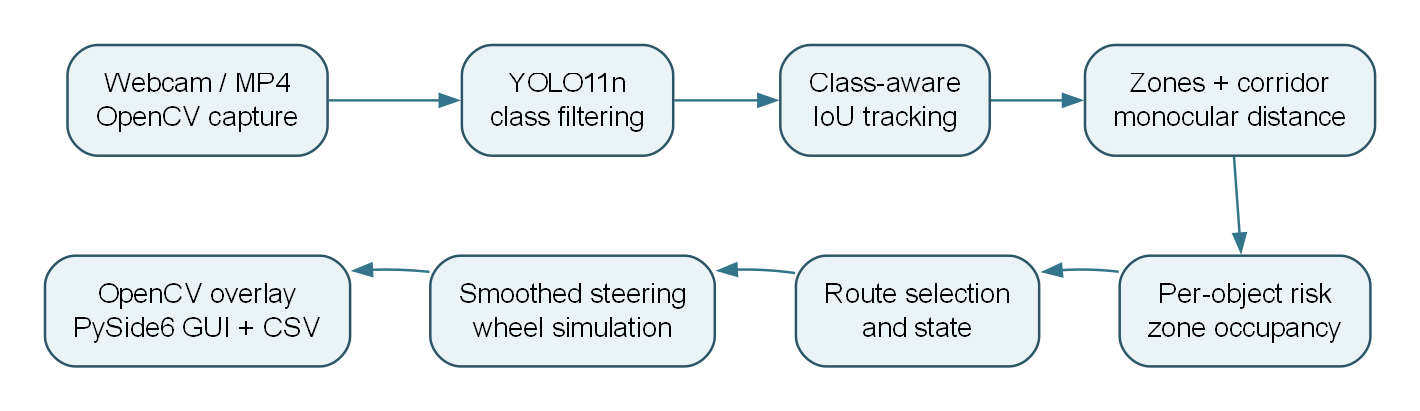
\includegraphics[width=0.92\textwidth]{system_flow.png}
  \caption{Implemented perception-to-decision path. The wheel values and trajectory are simulations. Diagram generated from the project's module structure.}
  \label{fig:pipeline}
\end{figure*}

\subsection{Data and Investigation Procedure}
The available repeatable input is a 24-second synthetic MP4 generated by the repository. It contains clear-path, approaching-center, side-obstacle, and blocked-path drawings. It is used to test playback, rendering, and timing rather than detector accuracy. A separate controlled capture script injects known detection boxes over this video to verify the downstream tracker, risk, decision, and GUI path. No labeled real-footage evaluation set, survey, or calibrated range measurements has yet been gathered.

The investigation has combined source review, deterministic unit tests, sampling of the synthetic video with the installed model, and inspection of actual Qt dashboard captures. Tests exercise an empty scene, lower-risk side selection, blocked-side emergency classification, zone boundaries, wheel direction, and steering clamp. The repository report and proposal record the full implementation and screenshot provenance \cite{projectdocs}.

\subsection{Preliminary Results}
On 3 October 2026, \texttt{python -m pytest -q} passed all six existing navigation tests. The included \texttt{yolo11n.pt} model loaded with CPU status. At 2, 6, 11, 16, and 21 seconds in the synthetic MP4, the detector returned zero objects. This finding limits the video to a GUI and logic fixture; it cannot demonstrate YOLO recognition performance. In contrast, controlled injected boxes produced the expected left-turn and blocked-route stop displays through the normal downstream pipeline. The displayed stop occurs immediately in that capture because the capture script sets the action hold to zero; normal configuration uses a 0.35-second minimum action duration.

\begin{figure*}[!t]
  \centering
  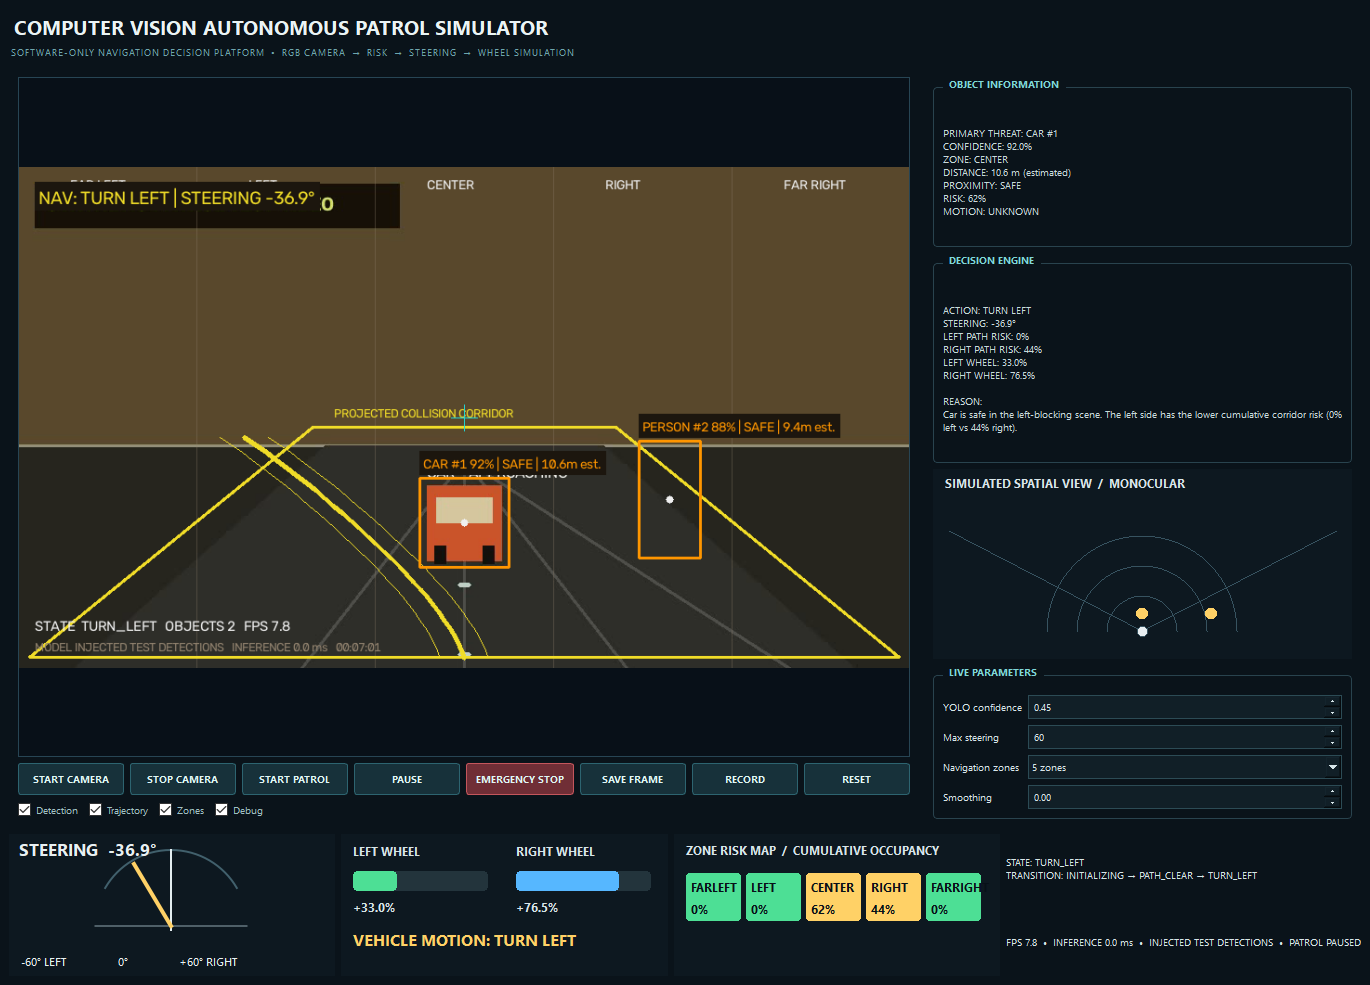
\includegraphics[width=0.76\textwidth]{dashboard_turn_left.png}
  \caption{Actual dashboard capture of a controlled left-turn case. Detection boxes were injected over synthetic video; this is evidence of navigation logic and visualization, not YOLO detection accuracy.}
  \label{fig:gui}
\end{figure*}

\section{Planned Work and Calendar Timeline}
The final project deadline supplied for this report is 4 October 2026. The short remaining window calls for focused validation and clear reporting, rather than a new model-training effort. Table~\ref{tab:timeline} separates completed work from the immediate submission tasks.

\begin{table}[!t]
\caption{Schedule to final submission}
\label{tab:timeline}
\centering
\footnotesize
\setlength{\tabcolsep}{3pt}
\begin{tabular}{|p{0.18\columnwidth}|p{0.42\columnwidth}|p{0.29\columnwidth}|}
\hline
\textbf{Date} & \textbf{Task} & \textbf{Evidence}\\ \hline
3 Oct 2026 & Freeze implementation baseline; run navigation tests; compile preliminary report. & Six passing tests and PDF draft.\\ \hline
4 Oct 2026 morning & Try YOLO-enabled inference on available real footage; record classes, misses, model status, and frame timing. & Short observation table with input and settings.\\ \hline
4 Oct 2026 afternoon & Rehearse clear, turn, and blocked demos; check labels and known limitations; submit source and final documents. & Reproducible demo and packaged report.\\ \hline
\end{tabular}
\end{table}

If suitable real footage cannot be obtained in time, the final submission will label that evaluation as incomplete rather than substitute synthetic detections. The proposed success criteria are a reproducible launch, passing existing tests, correct decision behavior for controlled scenes, and an honest account of inference behavior and limitations. Larger revisions such as calibrated depth or a worker thread for inference remain future work.

\section{Current Risks and Limitations}
The principal technical uncertainty is the monocular distance estimate. Unknown real object height, partial boxes, camera tilt, and lens properties can change the estimate; the project has not calibrated the camera. The displayed trapezoidal corridor differs from the center-rectangle geometry used in analysis. An inference exception currently yields an empty detection list, which can resemble a clear scene. The action hold may delay a requested stop, while the manual emergency override zeros the simulated wheels on the next processed frame without synchronizing the state history. Finally, the GUI timer runs inference in the GUI thread, so slow inference can reduce responsiveness. These findings define the interpretation of the preliminary results and the priority of future fixes.

\section{Conclusion}
The implemented prototype already demonstrates the complete capture-to-explanation software chain and passes the six available navigation tests. Its strongest contribution is visibility into how detection, approximate scene geometry, and configurable risk rules produce a simulated steering choice. The remaining work before the stated deadline is a small real-footage check, final demonstration verification, and careful packaging. The report does not claim validated detection accuracy, measured depth, or safe physical autonomy.

\begin{thebibliography}{00}
\bibitem{yolo11} G. Jocher and J. Qiu, ``Ultralytics YOLO11,'' Ultralytics, 2024. [Online]. Available: \url{https://docs.ultralytics.com/models/yolo11/}. Accessed: Oct. 3, 2026.
\bibitem{coco} T.-Y. Lin \emph{et al.}, ``Microsoft COCO: Common objects in context,'' in \emph{Proc. European Conf. Computer Vision}, 2014, pp. 740--755. [Online]. Available: \url{https://arxiv.org/abs/1405.0312}.
\bibitem{sort} A. Bewley, Z. Ge, L. Ott, F. Ramos, and B. Upcroft, ``Simple online and realtime tracking,'' in \emph{Proc. IEEE Int. Conf. Image Processing}, 2016, pp. 3464--3468. [Online]. Available: \url{https://arxiv.org/abs/1602.00763}.
\bibitem{opencvcalib} OpenCV, ``Camera calibration,'' OpenCV documentation. [Online]. Available: \url{https://docs.opencv.org/5.0/main_modules/calib.html}. Accessed: Oct. 3, 2026.
\bibitem{pyside} The Qt Company, ``Qt for Python,'' Qt documentation. [Online]. Available: \url{https://doc.qt.io/qtforpython-6/}. Accessed: Oct. 3, 2026.
\bibitem{projectdocs} C. Singh, ``Computer Vision Autonomous Patrol Simulator: Engineering analysis and demonstration report,'' project repository, Oct. 2026, \texttt{docs/PROJECT\_REPORT.md}.
\end{thebibliography}

\appendices
\section{Supplementary Technical Documents}
The repository provides \texttt{README.md} for installation and operation, \texttt{config.yaml} for default parameters, \texttt{docs/PROJECT\_REPORT.md} for detailed code analysis, \texttt{docs/PROJECT\_PROPOSAL.md} for the presentation concept, \texttt{tests/test\_navigation.py} for the six unit tests, and \texttt{docs/assets/} for the architecture and GUI figures. The synthetic test video is generated by \texttt{tools/create\_sample\_video.py}. No preliminary human survey was performed.

\section{Reproduction Commands}
From the repository root, install \texttt{requirements.txt}, run \texttt{python -m pytest -q}, generate the sample with \texttt{python tools/create\_sample\_video.py}, and launch \texttt{python main.py --video recordings/sample\_patrol.mp4 --no-model}. Use a real video or webcam with the model enabled to investigate detection. Run \texttt{python docs/build\_preliminary\_report.py} to regenerate this PDF from its \LaTeX{} source.

\end{document}
